%----------------------------------------------------------
\subsection{Color Space}
As described previously, in order to extract objects from the scene, the algorithm simplifies the color of every frame in several clusters of colors. To do that, thresholds on color channels were applied. But Firstly the used color space must be defined. \\
RGB is the most common color space, it's composed by three channels (One per color Red, Green and Blue). The main trouble using RGB frames is that objects color can change drastically, and threshold are worst limited (Color depend on three variable so limits between them are not flat surface but curved surface).
Instead of using RGB, in this project, HSV color space are chosen. HSV (Hue, Saturation and Value) has all the color information arrange in only one variable: H or Hue channel. That issue, simplifies the algorithm by making the color separation surfaces flats.  \\

% HSV vs RGB figure
\begin{figure}
	\centering
	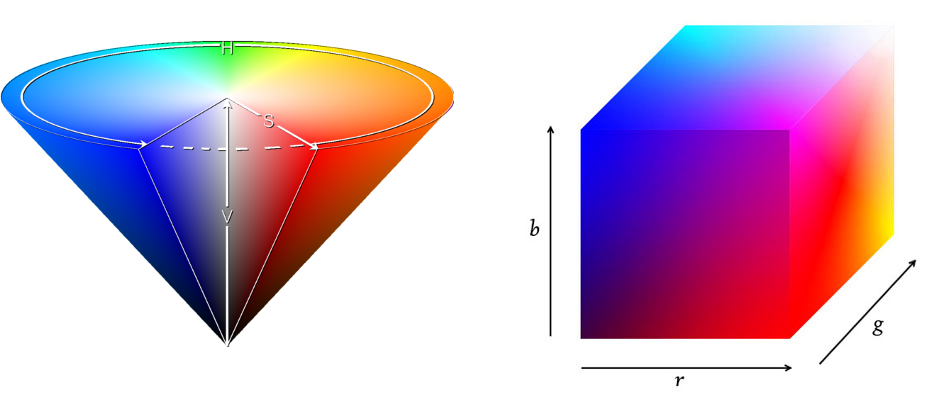
\includegraphics[width=0.75\textwidth,natwidth=944,natheight=400]{../Images/c1/HSV_vs_RGB.png}
	\caption{HSV and RGB spaces of color}
	\label{fig:HSV_vs_RGB}
\end{figure}

%----------------------------------------------------------
\subsection{Pixel Transformation}
Pixel Transformation method refers to the method which takes every single pixel of the image and transform it to a simplified color. That's made by applying a threshold the value of H, S and V channels. \\

\begin{wrapfigure}{r}{0.4\textwidth}
	\vspace{-2.5cm}
	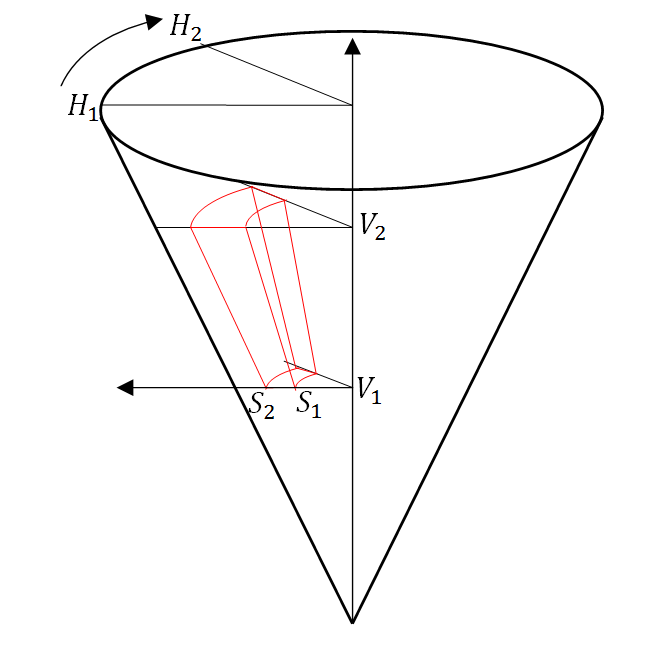
\includegraphics[width=0.4\textwidth,natwidth=659,natheight=659]{../Images/c1/DividingSubSpace.png}
	\caption{Division of subspace}
	\label{fig:DividingSubSpace}
\end{wrapfigure}

The common way to apply that threshold if by calling "if...else..." sentences. But that way is not very efficient. Images are commonly stored in the memory as arrays of 3-bytes (One byte per channel). Every channel has a value between 0 and 255, so that It's possible to use bitwise operations \cite{JamesBruce} that are so much faster than breaking the ""processor's pipeline"" with conditional sentences. \\

%%% 666 TODO: hablar de los limites y todo eso

In this document colors are grouped in eight clusters \{ Black, white, Blue, Purple, Red, Orange, Yellow, Green \} which frontiers are defined by ..... % 666 TODO: continue

%% 666 TODO: HABLAR DE LOS THRESHOLD LUEGO DE AGRUPARLOS TODOS PARA ACELERAR EL PROCESO QUITANDO LOS IFs.
%%%%% VENTAJAS: VELOCIDAD
%%%%% DESVENTAJAS: RESOLUCION

%----------------------------------------------------------
\subsection{Run-length encoding}
Run-length encoding or RLE is a simple form of data compression in which every groups or "runs" of data is compressed by and amount of pairs of data value and count. For example, having the following "runs": \\

\textit{WWWWWWWBBBBBBBBBCCCCCCWWWWWWWWWWWWWWWW} \\

The RLE algorithm will compress it to: \\
\textit{W7B9C6W16}

In this document, RLE is used to reduce image sizes allowing the segmentation algorithm to gather groups of colors and to go over the objects detected in the scene in a simple and fast iteration. \\

This kind of data compress is very useful and effective if the color in the picture is homogeneous. However, if not it could be contra-productive since can make the size of the "runs" grow. Here is an example of both cases: \\

%% 666 TODO: error en la lista....
%\begin{enumerate}
%	\item Homogeneous runs: \texit{WWWWWWWWWWWWWWWWWWWWWWWWWWWWWW \longrightarrow W30} \\
%	\item Heterogeneous runs: \textit{WAWAWAWAWAWAWAWA \longrightarrow W1A1W1A1W1A1W1A1W1A1W1A1W1A1W1A1} \\
%\end{enumerate}


%----------------------------------------------------------
\subsection{Object creation}
